% We need layers to draw the block diagram
\pgfdeclarelayer{background}
\pgfdeclarelayer{foreground}
\pgfsetlayers{background,main,foreground}

% Define a few styles and constants
\tikzstyle{sensor}=[draw, fill=blue!20, text width=5em, 
    text centered, minimum height=2.5em,rounded corners]
\tikzstyle{output}=[coordinate]
\tikzstyle{input}=[coordinate]
\tikzstyle{naveqs} = [sensor, text width=5em, fill=red!20, 
    minimum height=6em, rounded corners]
\def\blockdist{2.3}
\def\edgedist{1.1}
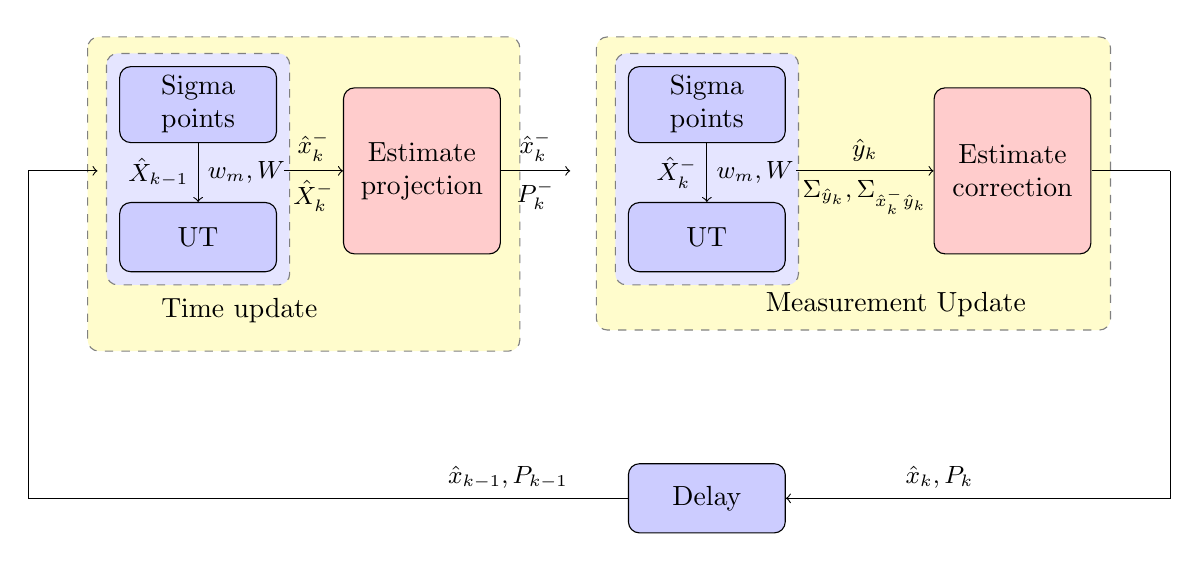
\begin{tikzpicture}[scale=0.8]
% Prediction block
    \node (xk)[input]{};
	\node (project) [naveqs,right of=xk,node distance=5cm]{Estimate projection};
	\path (project.140)+(-\blockdist,0) node (sigmapredict) [sensor] {Sigma points};
	\path (project.-140)+(-\blockdist,0) node (naveq) [sensor] {UT};
	\node (ut_project)[output, left of=project, node distance=1.75cm]{};
    \draw [->] (sigmapredict.south) -- node [left] {\small ${\hat{X}_{k-1}}$} node[right]{\small $w_m,W$}(naveq.north);
	\draw [->](ut_project.east) --node[above]{\small ${\hat{x}_k^-}$}node[below]{\small ${{\hat{X}^-_k}}$}(project.west);
    \path (naveq.south east)+(-0.6,-0.6) node (predict){Time update};
    
% Correction block
	\node (correct) [naveqs,right of=project,node distance=7.5cm]{Estimate correction};
	\path (correct.140)+(-3.6,0) node (sigmacorrect) [sensor] {Sigma points};
	\path (correct.-140)+(-3.6,0) node (ut) [sensor] {UT};
	\node (ut_correct)[output, left of=correct, node distance=2.75cm]{};
	\draw [->] (sigmacorrect.south) -- node [left] {\small ${\hat{X}_{k}^-}$} node[right]{\small $w_m,W$}(ut.north);
	\draw [->](ut_correct.east) --node[above]{\small ${\hat{y}_k}$}node[below]{\small ${\Sigma_{\hat{y}_k}},{\Sigma_{\hat{x}_k^- \hat{y}_k}}$}(correct.west);
    \path (correct.south west)+(-0.6,-0.8) node (msr_upd){Measurement Update};
	     
% Draw edges connecting prediction and correction blocks
    \draw [->] (project.east) -- node [above] {\small $\hat{x}^-_{k}$ }node [below] {\small $P_{k}^-$ } + (\edgedist,0); 
        node[right]{};
        
%	Draw the delay node below the other two nodes
	\node (delay) [sensor,below of=sigmacorrect,yshift =-4cm]{Delay};
	\node [output,right of=correct,xshift=1cm](out){};
	\draw [-] (correct.east) --(out);
    \draw [->] (out) |- node [above,pos=0.8]{\small $\hat{x}_k,P_k$}(delay);
    	\draw [->] (xk.east) --node{}+(\edgedist,0); node[right]{}; (sigmapredict.west);
    \draw [-](delay) -|node [above,pos=0.1]{\small $\hat{x}_{k-1},P_{k-1}$} (xk);

       \begin{pgfonlayer}{background}
        % Compute a few helper coordinates
        \path (sigmapredict.west |- project.north)+(-0.5,0.8) node (a) {};
        \path (predict.south -| project.east)+(+0.3,-0.3) node (b) {};
        \path[fill=yellow!20,rounded corners, draw=black!50, dashed]
            (a) rectangle (b);
        \path (sigmacorrect.west |- correct.north)+(-0.5,0.8) node (a) {};
        \path (correct.south -| correct.east)+(+0.3,-1.2) node (b) {};
        \path[fill=yellow!20,rounded corners, draw=black!50, dashed]
            (a) rectangle (b);
	   %Inner block predictor
       \path (sigmapredict.north west)+(-0.2,0.2) node (a) {};
       \path (naveq.south -| sigmapredict.east)+(+0.2,-0.2) node (b) {};
       \path[fill=blue!10,rounded corners, draw=black!50, dashed]
           (a) rectangle (b);
	   %Inner block corrector
       \path (sigmacorrect.north west)+(-0.2,0.2) node (a) {};
       \path (ut.south -| sigmacorrect.east)+(+0.2,-0.2) node (b) {};
       \path[fill=blue!10,rounded corners, draw=black!50, dashed]
           (a) rectangle (b);
       % \path (gyros.north west)+(-0.2,0.2) node (a) {};
       % \path (IMU.south -| gyros.east)+(+0.2,-0.2) node (b) {};
       % \path[fill=blue!10,rounded corners, draw=black!50, dashed]
        %    (a) rectangle (b);
    \end{pgfonlayer}
\end{tikzpicture}